\usepackage{xcolor}
\usepackage{afterpage}
\usepackage{pifont,mdframed}
\usepackage[bottom]{footmisc}
\usepackage{multicol}

\createsection{\Grader}{Grader di prova}
\createsection{\Detail}{Dettagli}

\renewcommand{\inputfile}{\texttt{stdin}}
\renewcommand{\outputfile}{\texttt{stdout}}
\makeatletter
\renewcommand{\this@inputfilename}{\texttt{stdin}}
\renewcommand{\this@outputfilename}{\texttt{stdout}}
\makeatother

\newenvironment{warning}
  {\par\begin{mdframed}[linewidth=2pt,linecolor=gray]%
    \begin{list}{}{\leftmargin=1cm
                   \labelwidth=\leftmargin}\item[\Large\ding{43}]}
  {\end{list}\end{mdframed}\par}
\newenvironment{danger}
{\par\begin{mdframed}[linewidth=2pt,linecolor=red!60!yellow,backgroundcolor=red!20!white]%
		\begin{list}{}{\leftmargin=1cm
				\labelwidth=\leftmargin}\item[\Large\ding{45}]}
		{\end{list}\end{mdframed}\par}

% % % % % % % % % % % % % % % % % % % % % % % % % % % % % % % % % % % % % % % % % % %
% % % % % % % % % % % % % % % % % % % % % % % % % % % % % % % % % % % % % % % % % % %

A gara terminata, i $P$ partecipanti delle Olimpiadi Italiane di Informatica
(numerati da $0$ a $P-1$) parteciperanno ad una cena di gala in piena tradizione
molisana.

Il banchetto consiste di $S$ piatti numerati da $0$ a $S-1$, ciascuno contenente
una tra le ``migliori 100 pietanze molisane'' scelte personalmente dallo chef:
la \emph{composta molisana}, lo \emph{spezzatino di pecora}, l'\emph{agnello con
cicoria} e altre $97$ succulente specialità.

Al momento dell'arrivo alla cena di gala i partecipanti si recheranno uno alla
volta verso l'inizio del banchetto, da destra verso sinistra (dal piatto $S-1$
verso il piatto $0$) e potranno scegliere se sedersi o se passare al piatto
successivo. Ogni partecipante ha una pietanza preferita, per cui si siederà al
banchetto solo in uno dei posti dove è apparecchiato un piatto contenente tale
pietanza. I partecipanti arrivano al banchetto in ordine dal primo all'ultimo
classificato.

Non è permesso scavalcarsi, quindi quando un partecipante decide di sedersi di
fronte al piatto $i$-esimo, tutti i piatti in posizione $j < i$ saranno
inaccessibili ai partecipanti seguenti. Una volta seduti, quindi, i partecipanti
avranno lo stesso ordine in cui sono arrivati. È possibile che ci siano dei
``buchi'' dove nessuno è seduto. I partecipanti non sono obbligati a scegliere
il primo piatto ``preferito'' che incontrano: tra i piatti contenenti la loro
pietanza preferita, infatti, \emph{possono sceglierne uno qualsiasi} come in figura.

\begin{figure}[H]%
	\centering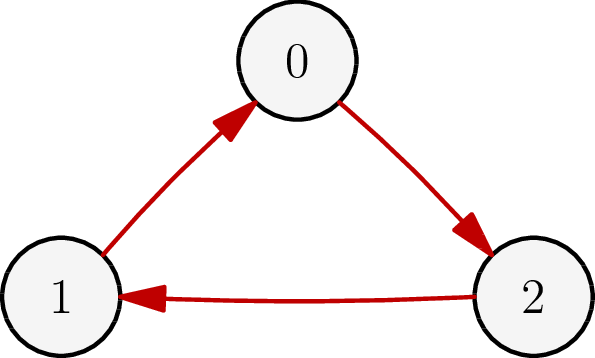
\includegraphics[width=\linewidth]{asy_cena/fig1.pdf}
\end{figure}

Purtroppo però è sorto un problema: Mojito e Chupito, rispettivamente il cane ed
il gatto di Monica, hanno eluso la sicurezza e si sono intrufolati nella sala
del banchetto prima dell'arrivo dei partecipanti. I due monelli sono saliti
sulla lunga tavolata con l'intenzione di papparsi alcuni dei piatti, in
particolare:
\begin{itemize}[nolistsep]
	\item Mojito è salito dal lato \emph{sinistro} del tavolo, per papparsi i
	piatti partendo dal numero $0$.
	\item Chupito è salito dal lato \emph{destro} del tavolo, per papparsi i
	piatti partendo dal numero $S-1$.
\end{itemize}

Monica, allertata dall'assenza dei suoi due pelosetti, è corsa verso il
banchetto e deve ora decidere come e quando fermare i due affamati. È possibile
fermare Mojito e Chupito in qualunque punto, anche prima che i due comincino a
mangiare. Tuttavia, intenerita dai suoi cuccioli, Monica vorrebbe lasciarli lì a
mangiare almeno un po' se possibile\dots

Indichiamo con $A$ e $B$ rispettivamente il numero di piatti mangiati da Mojito
e da Chupito. Aiuta Monica calcolando \textbf{quante coppie diverse} $(A, B)$
esistono tali che, anche ``sacrificando'' i primi $A$ piatti e gli ultimi $B$
piatti della lunga tavolata, \textbf{c'è almeno una strategia} che permette ai
partecipanti di sedersi tutti davanti ad un piatto contenente la propria
preferenza.

\begin{danger}
	\textbf{Nota bene:} i partecipanti delle OII sono curiosi di
	``sperimentare'' le pietanze molisane. Infatti, indipendentemente dal valore
	di $P$, il numero di partecipanti \emph{con una stessa pietanza preferita}
	non sarà mai superiore a \textbf{1000}.
\end{danger}

% % % % % % % % % % % % % % % % % % % % % % % % % % % % % % % % % % % % % % % % % % %
% % % % % % % % % % % % % % % % % % % % % % % % % % % % % % % % % % % % % % % % % % %

\Implementation

Dovrai sottoporre un unico file, con estensione \texttt{.c} o \texttt{.cpp}.

\begin{warning}
Tra gli allegati a questo task troverai un template \texttt{cena.c} e \texttt{cena.cpp}
con un esempio di implementazione.
\end{warning}

Dovrai implementare la seguente funzione:

\begin{center}\begin{tabularx}{\textwidth}{|c|X|}
\hline
C/C++  & \verb|long long conta(int S, int s[], int P, int p[]);|\\
\hline
\end{tabularx}\end{center}

\begin{itemize}[nolistsep]
  \item L'intero $S$ indica il numero di piatti nella tavola.
  \item L'array $s$ (indicizzato da $0$ a $S-1$) indica il tipo di cibo nell'$i$-esimo piatto.
  \item L'intero $P$ indica il numero di partecipanti.
  \item L'array $p$ (indicizzato da $0$ a $P-1$) indica la preferenza dell'$i$-esimo partecipante.
\end{itemize}

Il grader chiamerà la funzione \texttt{conta} e ne stamperà il valore restituito
sul file di output.

% % % % % % % % % % % % % % % % % % % % % % % % % % % % % % % % % % % % % % % % % % %
% % % % % % % % % % % % % % % % % % % % % % % % % % % % % % % % % % % % % % % % % % %


\Grader
Nella directory relativa a questo problema è presente una versione semplificata
del grader usato durante la correzione, che potete usare per testare le vostre
soluzioni in locale. Il grader di esempio legge i dati da \inputfile{}, chiama
le funzioni che dovete implementare e scrive su \outputfile{}, secondo il
seguente formato.

Il file di input è composto da tre righe, contenenti:
\begin{itemize}[nolistsep,itemsep=2mm]
\item Riga $1$: gli interi $S$ e $P$.
\item Riga $2$: i valori \texttt{s[$i$]} per $i = 0\ldots S-1$.
\item Riga $3$: i valori \texttt{p[$i$]} per $i = 0\ldots P-1$.
\end{itemize}

Il file di output è composto da un'unica riga, contenente:
\begin{itemize}[nolistsep,itemsep=2mm]
\item Riga $1$: il valore restituito dalla funzione \texttt{conta}.
\end{itemize}

% % % % % % % % % % % % % % % % % % % % % % % % % % % % % % % % % % % % % % % % % % %
% % % % % % % % % % % % % % % % % % % % % % % % % % % % % % % % % % % % % % % % % % %


\Constraints

\begin{itemize}[nolistsep, itemsep=2mm]
	\item $1 \le P \le S \le 100\,000$.
	\item $1 \le P \le 50\,000$.
	\item $0 \le \texttt{s[$i$]}, \texttt{p[$i$]} < 100$.
	\item Non esistono $1001$ partecipanti con la stessa preferenza.
\end{itemize}

% % % % % % % % % % % % % % % % % % % % % % % % % % % % % % % % % % % % % % % % % % %
% % % % % % % % % % % % % % % % % % % % % % % % % % % % % % % % % % % % % % % % % % %


\Scoring

Il tuo programma verrà testato su diversi test case raggruppati in subtask.
Per ottenere il punteggio relativo ad un subtask, è necessario risolvere correttamente tutti i test che lo compongono.

\begin{itemize}[nolistsep,itemsep=2mm]
  \item \textbf{\makebox[2cm][l]{Subtask 1} [\phantom{1}0 punti]}: Casi d'esempio.
  \item \textbf{\makebox[2cm][l]{Subtask 2} [13 punti]}: $S \leq 100$ e $P\le 100$. % O(S³)
  \item \textbf{\makebox[2cm][l]{Subtask 3} [23 punti]}: $P\le 1000$ e tutti i partecipanti hanno la stessa preferenza.
  \item \textbf{\makebox[2cm][l]{Subtask 4} [27 punti]}: $S \leq 10\,000$ e $P \le 100$. % O(S²P)
  \item \textbf{\makebox[2cm][l]{Subtask 5} [16 punti]}: $P\le 100$. % O(SP)
  \item \textbf{\makebox[2cm][l]{Subtask 6} [21 punti]}: Nessuna limitazione specifica. % O(SA)
\end{itemize}

% % % % % % % % % % % % % % % % % % % % % % % % % % % % % % % % % % % % % % % % % % %
% % % % % % % % % % % % % % % % % % % % % % % % % % % % % % % % % % % % % % % % % % %


\Examples

\begin{example}
\exmpfile{cena.input0.txt}{cena.output0.txt}%
\exmpfile{cena.input1.txt}{cena.output1.txt}%
\end{example}

% % % % % % % % % % % % % % % % % % % % % % % % % % % % % % % % % % % % % % % % % % %
% % % % % % % % % % % % % % % % % % % % % % % % % % % % % % % % % % % % % % % % % % %


\Explanation

Il \textbf{primo caso di esempio} coincide con quello illustrato nel testo. Per
garantire ai partecipanti di potersi sedere, ci sono $4$ modi di fermare Mojito
e Chupito:

\begin{itemize}[nolistsep,itemsep=2mm]
	\item \texttt{0[\underline{0}1\underline{2}\underline{0}]1} -- Monica lascia mangiare $1$ piatto a Mojito e $1$ piatto a Chupito.
	\item \texttt{[0\underline{0}1\underline{2}\underline{0}1]} -- Mojito $0$ piatti, Chupito $0$ piatti.
	\item \texttt{[\underline{0}01\underline{2}\underline{0}]1} -- Mojito $0$ piatti, Chupito $1$ piatto.
	\item \texttt{0[\underline{0}1\underline{2}\underline{0}1]} -- Mojito $1$ piatto, Chupito $0$ piatti.
\end{itemize}

La zona ``risparmiata'' dai due affamati è indicata tra parentesi quadre.
Inoltre, per dimostrare che tutti questi modi garantiscono ai partecipanti di
trovare la propria pietanza preferita, è stata \underline{sottolineata} una
possibile disposizione che questi potrebbero scegliere.

Nel \textbf{secondo caso di esempio}, dato che i partecipanti hanno tutti la stessa
preferenza, sono validi tutti i modi di fermare Mojito e Chupito che
risparmiano almeno $3$ piatti di tipo \texttt{`0'}:

\setlength{\columnsep}{-2.1in}
\begin{multicols}{2}
	\begin{itemize}[nolistsep,itemsep=2mm]
		\item \texttt{[\underline{0}1\underline{0}11\underline{0}]101}
		\item \texttt{[\underline{0}1\underline{0}11\underline{0}1]01}
		\item \texttt{[01\underline{0}11\underline{0}1\underline{0}]1}
		\item \texttt{[\underline{0}1011\underline{0}1\underline{0}1]}

		\item \texttt{0[1\underline{0}11\underline{0}1\underline{0}]1}
		\item \texttt{0[1\underline{0}11\underline{0}1\underline{0}1]}
		\item \texttt{01[\underline{0}11\underline{0}1\underline{0}]1}
		\item \texttt{01[\underline{0}11\underline{0}1\underline{0}1]}
	\end{itemize}
\end{multicols}
